\chapter{Development of a Web Application Programming Interface for Genome Properties Data}

As discussed in Chapter XXX, one of core goals of Micromeda is to provide users with an interface for visualizing the presence and absence of genome properties across multiple organisms. The author chose to deliver this software in the form of a web application which takes Micromeda files and uses the data within to generate interactive heatmap-based visualizations. The use of a web application has several advantages and these are discussed in Chapter XXX. Due the inherent complexity of the information stored within Micromeda files, and some features requested such as the ability to download proteins sequences which support the existence of property steps, it was determined that both a web browser application and supporting server program, called Micromeda-Server, would have to be developed. In this chapter, we will discuss the sever component in detail, including the services it provides and its implementation. The author will discuss the web application that uses these services in the following Chapter XXX.

\section{Overview of Web Servers}

A widespread delivery mechanism for data analysis software, such as Micromeda, is via the World Wide Web \cite{berners1994world} and in the form of a web application. In such implementations, users connect to a remote server computer system \footnote{For this document, the term \textbf{server computer system} is used to refer to the physical hardware on which software is running. The term \textbf{server} is used to refer to a software process which provides users or applications with data. A server process may provide data directly to other processes running on the same server computer system or provide data over a network in response to a remote procedure call (RPC) \cite{nelson1981remote}.} via their web browser and download the code for the application. The application is then run within their browser. Such applications follow a client-server architecture \cite{svobodova1985client} (see \href{en.wikipedia.org/wiki/Client–server\_model}{en.wikipedia.org/wiki/Client–server\_model}) where the code running in the user's browser is called the client. If the client requires external data, it can request this information from a server process running on a server computer system. Clients can request different types of information from a server, including images, videos, files, and stored data. Requests to the server are made, via Hypertext Transfer Protocol (HTTP) \cite{fielding1999hypertext}, using a series of Uniform Resource Locator (URL) addresses \cite{berners1994rfc} (i.e., web addresses) that return specific types of data. These addresses are known as \textbf{endpoints} (Section \ref{endpoints}) and form an web Application Programming Interface (API) (see \href{en.wikipedia.org/wiki/Application\_programming\_interface}{en.wikipedia.org/wiki/Application\_programming\_interface}).

\section{Micromeda-Server Workflow and Implementation} \label{server-workflow}

\begin{figure}[!ht]
  \centering
	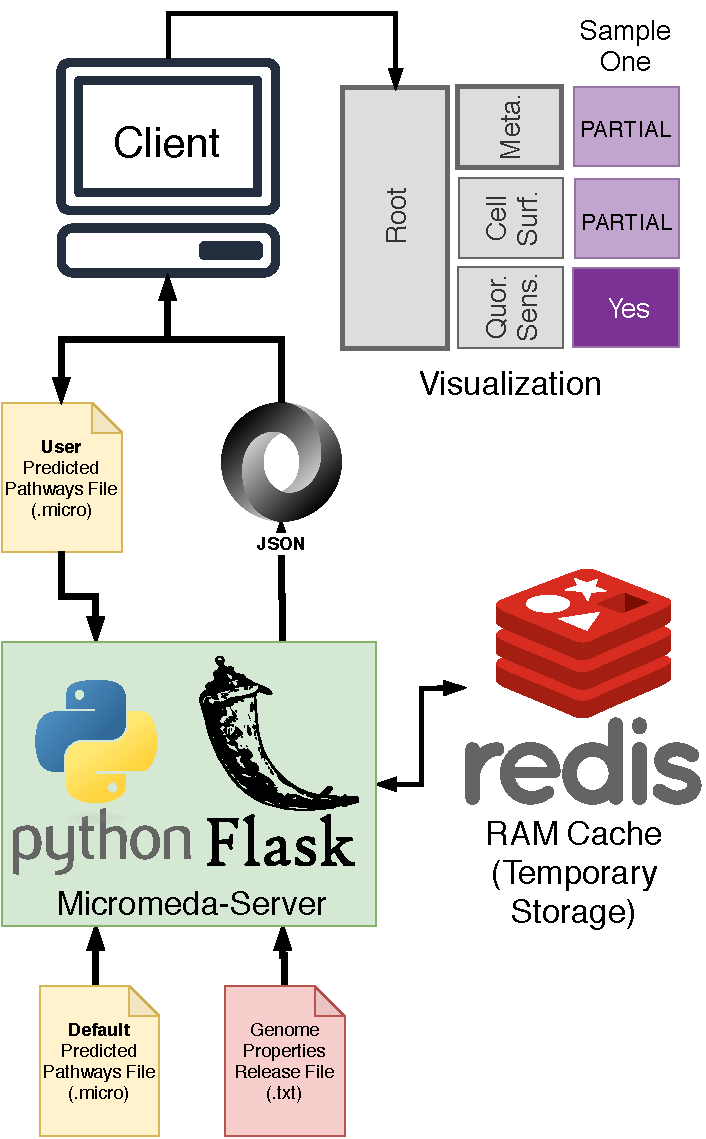
\includegraphics[width=0.60\textwidth]{media/Micromeda-Server.pdf}
	 \caption{Micromeda-Server consists of a server application written in Python using the Flask web framework. It is supported by a Redis caching server and series of text files. A genomeProperties.txt file supplies information about the Genome Properties DAG. Micromeda files, either default or uploaded, provide information about property assignments, step assignments and supporting information for multiple organisms.}
	 \label{fig:micromeda-server}
\end{figure}

\begin{figure}[!ht]
  \centering
	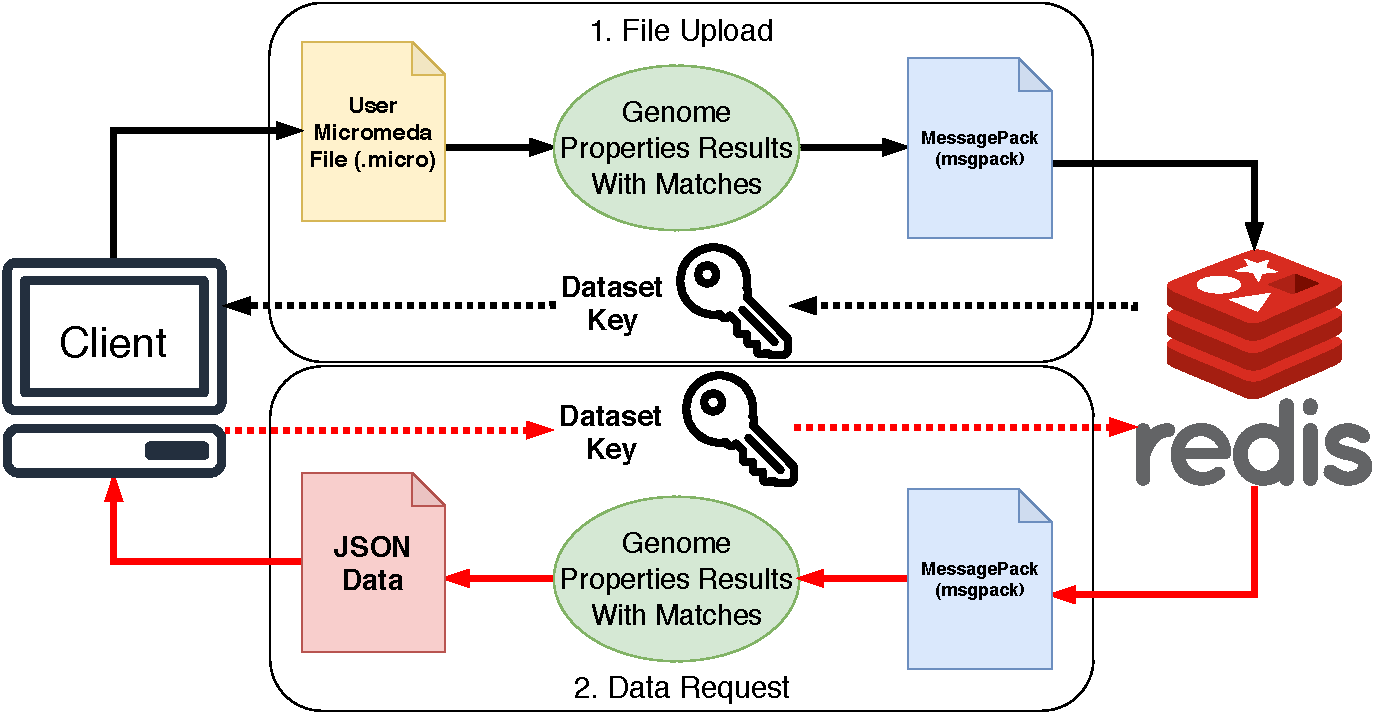
\includegraphics[width=0.80\textwidth]{media/Micromeda-Server-Workflow.pdf}
	 \caption{Micromeda-Server uses uploaded or default Micromeda files to generate GenomePropertiesResultsWithMatches objects. These instantiations are cached in Redis and reconstituted between API requests. Individual endpoints of Micromeda-Server use methods possessed by GenomePropertiesResultsWithMatches objects to produce responses that are sent to web client applications.}
	 \label{fig:micromeda-server-workflow}
\end{figure}

\begin{figure}[!ht]
  \centering
	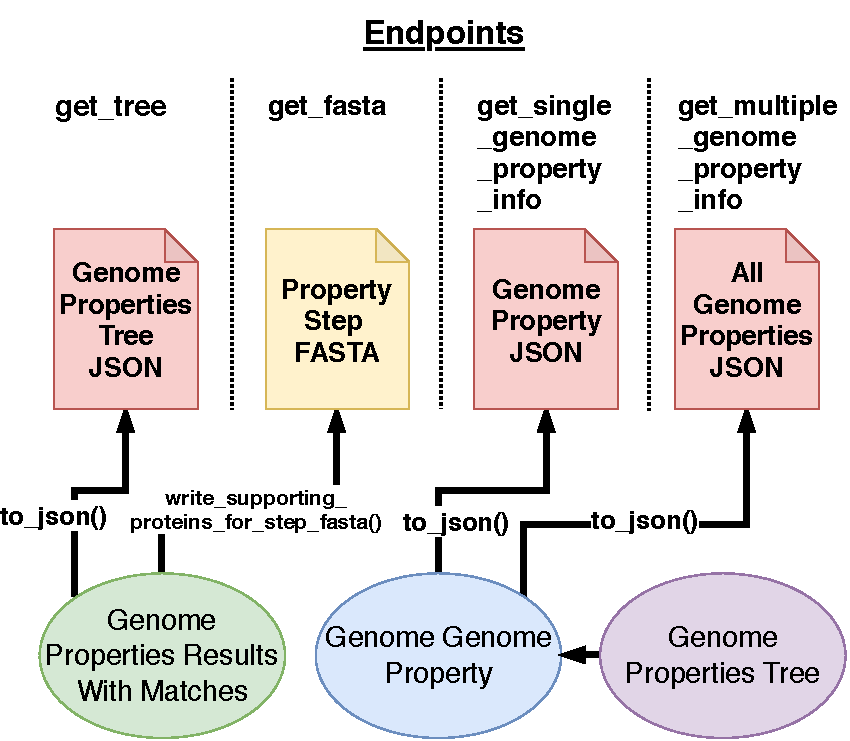
\includegraphics[width=0.70\textwidth]{media/Micromeda-Endpoints.pdf}
	 \caption{JSON documents and FASTA files for individual API endpoints are generated using methods of GenomePropertiesResultsWithMatches and the child GenomeProperty objects of GenomePropertiesTree objects.}
	 \label{fig:micromeda-endpoints}
\end{figure}

Micromeda-Server is designed to provide a web API to client applications that require access to information about the Genome Properties database. It also provides an API for accessing temporarily stored property assignments, step assignments and supporting information for user supplied datasets. It is written in Python and utilizes the Flask web development framework \cite{grinberg2018flask} (Fig. \ref{fig:micromeda-server}) to map Python functions for handling specific web API requests to server URL addresses. Information about the Genome Properties database is supplied to Micromeda-Server via a \textbf{genomeProperties.txt} release file (Fig. \ref{fig:micromeda-server} and Section \ref{genome-properties-files}). Property assignments, step assignments and supporting information for user datasets are supplied via user uploaded Micromeda files (Fig. \ref{fig:micromeda-server}). These Micromeda files are parsed into GenomePropertyResultsWithMatches objects (Subsection \ref{PropertyResultsWithMatches}) which are later stored in an in-memory Redis cache \footnote{Redis is an server process which provides a in-memory key-value store with hard-disk drive (HDD) back-up  \cite{han2011survey}. It allows for the caching of datasets in random-access memory (RAM). Each value stored can later be retrieved from Redis using a key provided during the caching process. These cached objects can even be accessed over the network by processes running in adjacent server computer systems. It can also be set up in a distributed cluster configuration across several server computer systems for redundancy and availability. Redis was chosen over competing caching servers such as Memcached \cite{fitzpatrick2004distributed} due to its ability to handle larger MessagePack binaries \cite{furuhashi2013messagepack} and its ability to back-up data to disk. Disk backup is important as it allows for the safe storage of datasets overtime and across high traffic volumes where the server may have ran out of RAM if Memcached was used.} in MessagePack format \cite{furuhashi2013messagepack} (Fig. \ref{fig:micromeda-server} and Fig. \ref{fig:micromeda-server-workflow}) (see Section \ref{msgpack}). In the context of Micromeda-Server, the contents of each uploaded and cached Micromeda file is referred to as a dataset. A single Micromeda file can also be provided to Micromeda-Server during start up for use as default dataset (Fig. \ref{fig:micromeda-server}). This default dataset is also parsed to a GenomePropertiesResultsWithMatches object and is used to supply data to the API if no Micromeda files are uploaded by users. The standard workflow for starting and using Micromeda-Server is the following:

\begin{enumerate}
  \item Start Micromeda-Server while providing a \textbf{genomeProperties.txt} file and an optional default dataset Micromeda file
  \item The \textbf{genomeProperties.txt} file is parsed to a GenomePropertiesTree object
  \item The default dataset Micromeda file is parsed to a GenomePropertiesResultsWithMatches object
  \item The client application sends a user supplied Micromeda file to the server via the upload endpoint
  \item The user supplied Micromeda files is parsed to a GenomePropertiesResultsWithMatches object which is later stored in the Redis cache in MessagePack format (Fig. \ref{fig:micromeda-server-workflow})
  \item The server supplies the client with a dataset key which is unique to each uploaded Micromeda file (Fig. \ref{fig:micromeda-server-workflow})
  \item The client can later supply this dataset key to the server during API requests to get information from previously uploaded Micromeda files (Fig. \ref{fig:micromeda-server-workflow})
  \item If no dataset key is provided by the client then the server supplies information about the default dataset during API requests
\end{enumerate}

Each GenomePropertiesResultsWithMatches object cached to Redis is given a Time To Live (TTL) value \cite{gwertzman1996world} (see \href{en.wikipedia.org/wiki/Time\_to\_live}{en.wikipedia.org/wiki/Time\_to\_live}). This value can be set to any time period such as minutes or days. After the TTL of the cached object is exceeded, it is flushed from the cache and the user will have to re-upload their Micromeda file. The default TTL used is two hours. During each API request, if a dataset key is provided, the MessagePack formatted GenomePropertiesResultsWithMatches object is grabbed from the cache and reconstituted into its original form (Fig. \ref{fig:micromeda-server-workflow}). During the API call this reconstituted GenomePropertiesResultsWithMatches object's method are used to supply data to the client  (Fig. \ref{fig:micromeda-server-workflow} and Fig. \ref{fig:micromeda-endpoints}). Further details on these endpoints are provided in Section \ref{endpoints}.

\section{Use of Redis for Dataset Caching} \label{redis-caching}

When developing Micromeda-Server the author had the choice of storing the information contained within upload Micromeda files permanently or temporarily. Do these files storage 

Python, due to limitations in its default cPython interpreter \cite{van1995python}, is only capable executing one thread at a time \cite{beazley2010understanding}. This causes problems for web server APIs which are required to handle multiple requests from clients simultaneously. In response, the majority of Python web frameworks, which provide boilerplate code for writing API endpoints, are designed to run multiple copies of the Python script which handles endpoint requests (Fig. \ref{fig:client-processing}). Flask is one such framework \cite{grinberg2018flask}. These scripts are run in separate processes and do not share a memory space (Fig. \ref{fig:client-processing}). Thus any objects data created in one is not shared with the others (Fig. \ref{fig:client-processing}). Also there is no guarantee that subsequent API requests from a single web client will be repeatedly mapped to the same API server process (Fig. \ref{fig:client-processing}). This lack of mapping causes problems as the object created for one client, for example a GenomePropertiesResultsWithMatches object created from the upload of a Micromeda file, would only be stored in one process and would not be available in other process that future client requests may be directed too (Fig. \ref{fig:client-processing}). One way of getting around this process isolation issue is to store data that needs to be shared between web server processes in an external process which is used to cache (Fig. \ref{fig:micromeda-server-workflow} and Fig. \ref{fig:client-processing}). This way the web API process have one place to call to get their shared data. In the case of Micromeda's server process we chose to use Redis as this caching process. Redis is a caching server that stores keyed data RAM. It also can be given memory use limits and will store store a portion of its data on disk. Micromeda's server use Redis to cache GenomePropertiesResultsWithMatches objects, in MessagePack format, for use by its many request handling processes (Fig. \ref{fig:micromeda-server-workflow}). These GenomePropertiesResultsWithMatches objects are generated from Micromeda files uploaded to the server. During API requests where the client wants data from a specific dataset, Micromeda's serve process pull MessagePack formatted GenomePropertiesResultsWithMatches objects from the Redis cache, reconstitute them and use their methods to gather data for the request (Fig. \ref{fig:micromeda-server-workflow}  and Fig. \ref{endpoints}). The very fast speed of serialization and deserialization of MessagePack to and from GenomePropertiesResultsWithMatches objects allows for this data-flow with minimal performance penalties (see Subsection \ref{messagepack-performance}).

\begin{figure}[!ht]
  \centering
	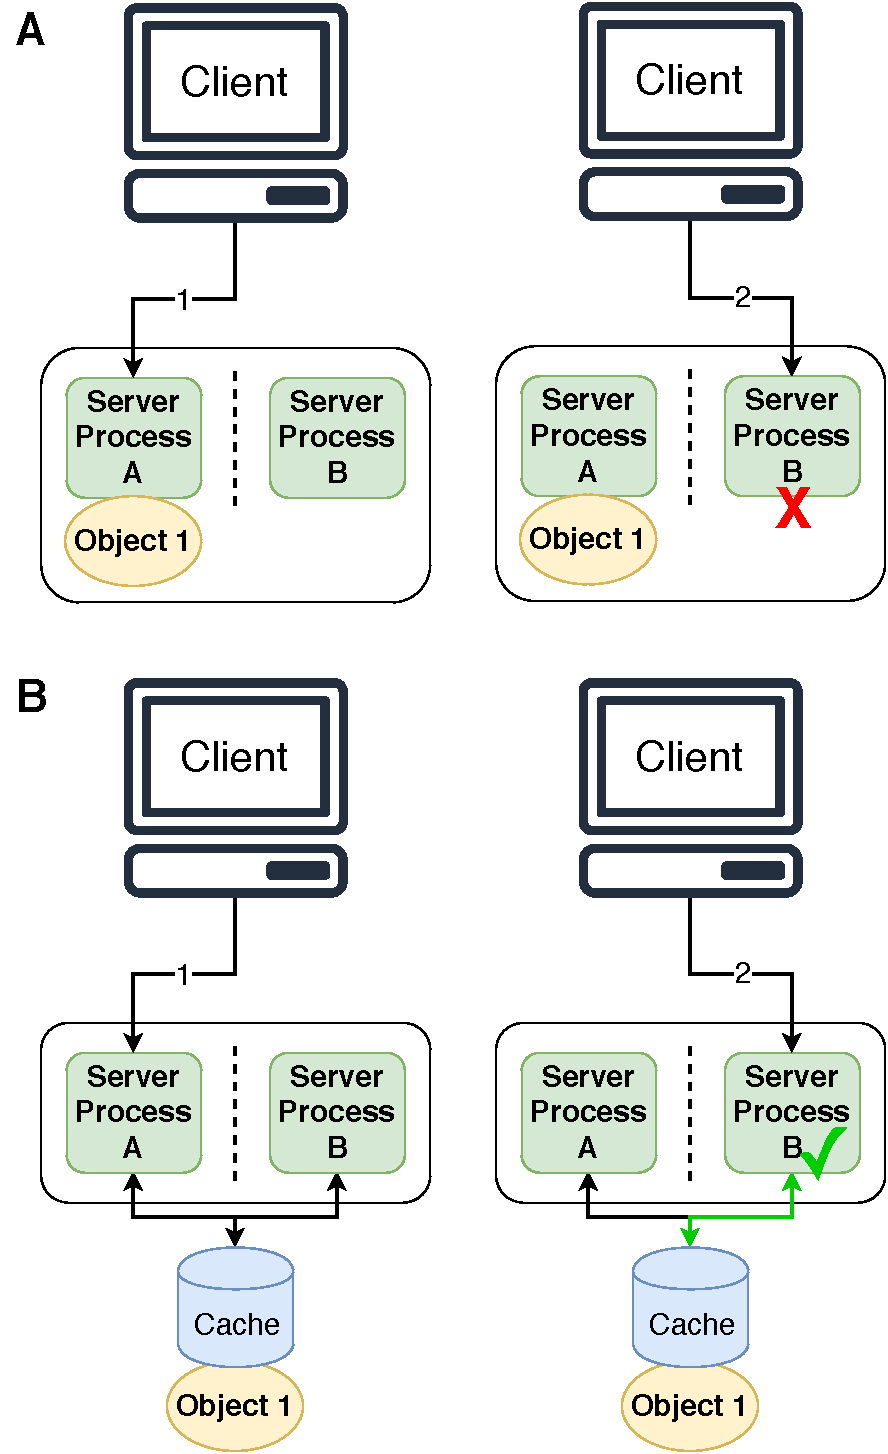
\includegraphics[width=0.60\textwidth]{media/Client-Processing.pdf}
	 \caption{Requests directed towards Python web APIs are spread out between a series of process. These processes cannot share data directly. Data to be shared between processes must be stored in a third process such as a cache or database.}
	 \label{fig:client-processing}
\end{figure}

\section{Application Programming Interface Endpoints} \label{endpoints}

Micromeda-Server provides several endpoints for supplying web clients with information about individual genome properties and information from uploaded Micromeda files. These endpoints were written using the Flask Python web framework \cite{grinberg2018flask} and are represented by \textbf{clean URLs} (see \href{en.wikipedia.org/wiki/Clean\_URL}{en.wikipedia.org/wiki/Clean\_URL}) where some information that would normally be stored as HTTP GET parameters are stored in the URL path (Fig. \ref{fig:endpoint-url}). Flask was chosen due to its simplicity as compared to more comprehensive frameworks such as Django \cite{holovaty2009definitive}. The endpoints also follow a representational state transfer (REST) architecture \cite{fielding2000representational} (see \href{en.wikipedia.org/wiki/Representational\_state\_transfer}{en.wikipedia.org/wiki/Representationa \_state\_transfer}). These endpoints and their implementation are summarized in Table \ref{tab:endpoints}, Fig. \ref{endpoints}, Fig. \ref{fig:endpoint-url} and detailed in subsections below.

\begin{figure}[!ht]
  \centering
	
\includegraphics[width=\textwidth]{media/Coloured-Endpoint.pdf}
	 \caption{The URL above is used to download a FASTA file for containing the top (i.e., those with lowest E-value domains) proteins which support GenProp0526 step one for dataset FXDABADS. The URL path variables are in blue and the HTTP GET parameters are in green.}
	 \label{fig:endpoint-url}
\end{figure}

\begin{longtable}{|p{1.6cm}|p{2.5cm}|p{1.4cm}|p{2.2cm}|p{2.2cm}|p{4cm}|}
\caption{Micromeda's server component provides web applications with five endpoints where they can request data about individual genome properties, upload Micromeda files and request information about stored assignment databases.}
\label{tab:endpoints}\\
\hline
\textbf{Python Function Name} & \textbf{Endpoint URL} & \textbf{HTTP Request Types} & \textbf{URL Path Variables} & \textbf{GET Parameter Variables} & \textbf{Return Value} \\ \hline
\endfirsthead
%
\multicolumn{6}{c}%
{{\bfseries Table \thetable\ continued from previous page}} \\
\hline
\textbf{Python Function Name} & \textbf{Endpoint URL} & \textbf{HTTP Request Types} & \textbf{URL Path Variables} & \textbf{GET Parameter Variables} & \textbf{Return Value} \\ \hline
\endhead
%
upload & /upload & GET, POST & None & None & JSON containing a dataset key that can be used in future requests to access information from the uploaded Micromeda file \\ \hline
get\_tree & /genome \_properties \_tree & GET & None & dataset\_key (optional) & A JSON tree representing all properties in the current Genome Properties database with each node annotated with a list of YES, NO, PARTIAL assignments for each sample \\ \hline
get\_single \_genome \_property \_info & /genome \_properties/ \textless{}string: property\_id\textgreater{} & GET & property\_id & None & JSON containing information about a genome property such as a description and a list of equivalent records from other databases (e.g. KEGG, MetaCyc) \\ \hline
get \_multiple \_genome \_property \_info & /genome \_properties & GET & None & None & A JSON array containing information about all genome properties in the database. Each property is given a description and a list of equivalent records from other databases (e.g. KEGG, MetaCyc) \\ \hline
get\_fasta & /fasta/ \textless{}string: property\_id\textgreater{}/ \textless{}int:step \_number\textgreater{} & GET & property\_id, step\_number & dataset\_key (optional), top (optional) & A FASTA file containing either all or the top proteins (i.e., those with lowest E-value domain annotation) supporting the existence of a given property step of a given dataset \\ \hline
\end{longtable}

\subsection{The Upload Endpoint} \label{endpoint-upload}

This API endpoint accepts the client upload of a Micromeda file and returns a hexadecimal encoded universally unique identifier (UUID) key \cite{leach2005universally} (see \href{en.wikipedia.org/wiki/Universally\_unique\_identifier}{en.wikipedia.org/wiki/ Universally\_unique\_identifier}) to the client. After upload, the Micromeda file is parsed and transformed into a GenomePropertiesResultsWithMatches object. This object is then serialized to MessagePack using the object's \textbf{to\_msgpack} function (Table \ref{tab:genomepropertyresultswithmatches})) and the resulting binary is cached in Redis using the Redis Python library \cite{mccurdy_2019} (Fig. \ref{fig:micromeda-server-workflow}). During the previous process a UUID, to be used as a dataset key, is generated using Python's builtin UUID generation function \cite{PythonUUID}. This UUID is used as the key for accessing the MessagePack serialization stored in the Redis cache (Fig. \ref{fig:micromeda-server-workflow}). It is also returned to the client application in response to the file upload. The client can provide this key to other API endpoints to receive data from the uploaded Micromeda file (Fig. \ref{fig:micromeda-server-workflow}). 

\subsection{The Get\_Tree Endpoint} \label{get-tree}

The Get\_Tree endpoint provides the client with a JSON tree representing all properties and steps in Genome Properties database (Fig. \ref{fig:tree-json}). This tree represents parent-child relationships between properties. Step nodes are also attached to their parent genome property nodes and act as leaves. Note that this endpoint returns a tree not a DAG (Fig. \ref{fig:tree-json}). In this tree, properties which would have had two parents in the Genome Properties DAG (Section XXX) are duplicated (Fig. fig:tree-json). Each property and step node in the tree is annotated by a list of assignments of support (i.e., YES, NO, PARTIAL), one for each sample in an previously uploaded or default Micromeda file (Fig. \ref{fig:tree-json}). The Get\_Tree endpoint can take a \textbf{dataset\_key} HTTP GET parameter variable (Table \ref{tab:endpoints}). If a dataset key generated by the previous upload of Micromeda file is assigned to this variable, then the assignments of support stored in the key's associated Micromeda file are used. The dataset key is used to reconstitute a GenomePropertiesResultsWithMatches object, representing the uploaded Micromeda file, from the Redis cache. The GenomePropertiesResultsWithMatches object's \textbf{to\_json} method (Table \ref{tab:genomepropertyresultswithmatches}) is called generate the above tree JSON returned from the endpoint. If no dataset\_key is provided, GenomePropertiesResultsWithMatches object of the default Micromeda is used to generate the tree JSON using the same method.

\begin{figure}[!ht]
  \centering
	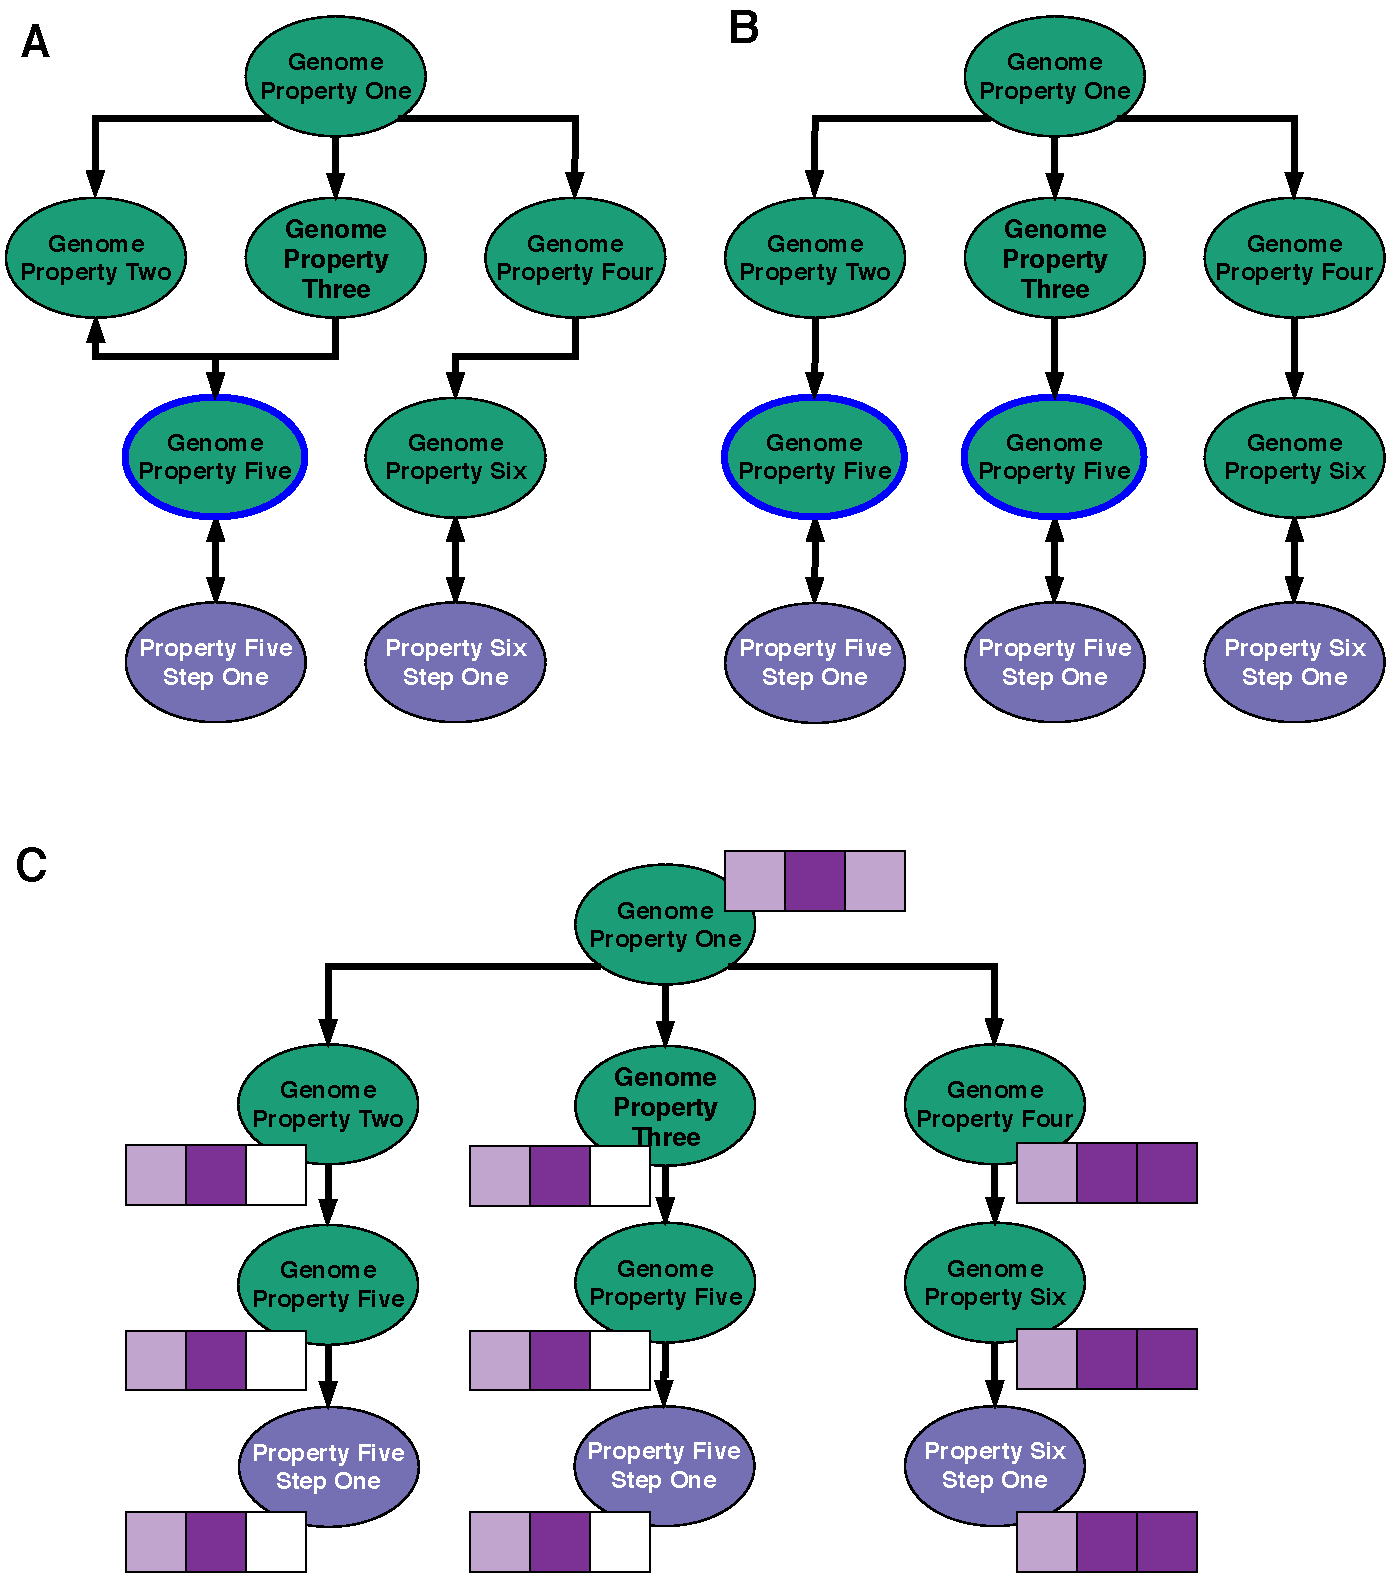
\includegraphics[width=0.70\textwidth]{media/Tree-JSON.pdf}
	 \caption{ (A and B) The JSON document created by the Get\_Tree endpoint forms a tree (right), not a DAG (left). (B) In this tree some nodes can be repeated. (C) In this JSON document each node is tagged with a list YES (Dark Purple), PARTIAL (Light Purple), and NO (White) assignments.}
	 \label{fig:tree-json}
\end{figure}


\subsection{The Get\_Single\_Genome\_Property\_Info Endpoint}

The Get\_Single\_Genome\_Property\_Info endpoint takes a genome property identifier as a URL parameter. This genome property identifier is used query for a matching GenomeProperty object (Section \ref{genome-property-class}), representing the property whose identifier is specified, from a global GenomePropertiesTree object (Section \ref{GenomePropertiesTree-Class}) created on Micromeda-Server's start (Section \ref{server-workflow}). If found, this GenomeProperty object's \textbf{to\_json} method (Table \ref{tab:genome-property-object}) is called to create a JSON document containing property information that is returned by the endpoint. This JSON document includes the property name, property description and a list of equivalent records from other databases (Table \ref{tab:genome-property-object}).

\subsection{The Get\_Multiple\_Genome\_Property\_Info Endpoint}

When the The Get\_Multiple\_Genome\_Property\_Info endpoint is called, the \textbf{to\_json} method (Table \ref{tab:genome-property-object}) is called for every GenomeProperty object (Section \ref{genome-property-class}) of the GenomePropertiesTree object (Section \ref{GenomePropertiesTree-Class}) created on Micromeda-Server start and each of the JSON strings generated placed into a list in a single larger JSON document which was returned by this endpoint. 

\subsection{The Get\_Fasta Endpoint} \label{get-fasta-endpoint}

The Get\_Fasta endpoint is used to send the client a FASTA file containing protein sequences which support the existence of a property step across multiple organisms and for a specific uploaded dataset. The URL path of requests to this endpoint include the genome property identifier and step number of the property step for which to generate a FASTA file. The FASTA file can either contain all proteins which support the existence of a step or only those who have the lowest E-value for the InterPro domain which supports the existence of a property step. These proteins are known as the \textbf{"top"} hits. The contents of the returned file is controlled by the presence of a HTTP GET parameter called \textbf{all} (Fig. \ref{fig:endpoint-url}). If all is set to true, then a FASTA file containing all proteins which support a step is returned. Otherwise, a FASTA file containing only the lowest E-value proteins is returned. Like the Get\_Tree endpoint, this endpoint also accepts a \textbf{dataset\_key} HTTP GET parameter (Fig. \ref{fig:endpoint-url}). The value this variable is used to reconstitute a GenomePropertiesResultsWithMatches object representing a previously uploaded Micromeda file (Fig. \ref{fig:micromeda-server-workflow}). This object's \textbf{write\_supporting\_proteins\_for\_step\_fasta} function (Table \ref{tab:genomepropertyresultswithmatches}) is used generate the FASTA file which is sent to the client.

\section{Micromeda Server Performance} \label{micromeda-server-performance}

The performance of Micromeda's endpoints was tested using a Micromeda file generated from the sequences and InterProScan annotations of the proteins of \textit{Chlorobium chlorochromatii} CaD3 (NCBI Taxonomy ID 340177) and \textit{Pelodictyon luteolum} DSM 273 (NCBI Taxonomy ID 319225). When this file was sent to the \textbf{upload} endpoint it was parsed and added to the Redis cache in 11.3s \textpm 2s. The \textbf{get\_tree} endpoint could create a genome property tree with assignment annotations from this cached Micromeda file in 9.4s \textpm 4s. The \textbf{get\_fasta} endpoint could generate a FASTA file with the top supporting proteins for GenProp0633 step number two in 33ms \textpm 4ms. Property information JSONs could be generated by the \textbf{get\_single\_genome\_property\_info} endpoint in 7ms \textpm 2ms. The \textbf{get\_multiple\_genome\_property\_info} can generated JSON for multiple properties in 23ms \textpm 5ms. The slow execution time of the \textbf{upload} and \textbf{get\_tree} endpoints was found to cause latency in client applications. For example, their is a noticeable delay in the rendering of visualizations in Micromeda's client application. Thus the performance of these endpoints should be optimized. Potential optimizations are discussed in Section \ref{micromeda-server-improvements}.

\section{Micromeda Server Deployments}

It is quite common to deploy web servers in different configurations depending on excepted request volume. Choosing the right configuration becomes even more important with Micromeda-Server as it is written using the Flask web framework \cite{grinberg2018flask}. Flask is single threaded and high performance can only achieved by running multiple copies of Micromeda-Server's Python script in parallel (as discussed in Section \ref{redis-caching}). These copies can be run on a single server or across a cluster of servers. Redis can also be run in a cluster configuration as well. In the below subsubsection three deployment strategies of increasing size will be discussed. 

\subsection{Development and Single User Deployment}

If a user chooses to install and run Micromeda-Server on their own desktop or laptop and only needs to visualize one dataset at time, then a vary simplified deployment strategy can be used. This deployment uses Flask's builtin development HTTP server that is created when the Micromeda-Server Python script is run directly. This sever is slow and can only handle requests from one client at a time. For this deployment Redis is not required and users must specify that Micromeda-Server uses the Micromeda file containing their dataset as a default dataset for Micromeda. In this mode the upload endpoint is turned off. This deployment method is similar to that used by Anvio's Metagenome Assembled Genome (MAG) visualization and refinement server \cite{eren2015anvi}. This deployment configuration is also useful for developer who want to test new features or bug fixes which they have added to Micromeda.

\begin{figure}[!ht]
  \centering
	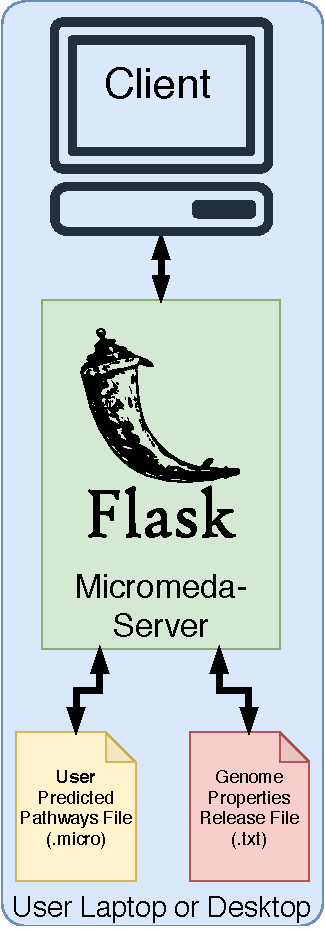
\includegraphics[width=0.30\textwidth]{media/micromeda-simple-deployment.pdf}
	 \caption{For the development use or deployment to laptop and desktops, Micromed-Server can use Flask's built in HTTP server, genomeProperties.txt file and a Micromeda file supplied on the server on start up.}
	 \label{fig:micromeda-small-deploy}
\end{figure}

\subsection{Single Server Deployment}

If a user requires Micromeda-Server to handle multiple users simultaneously, such as would be the case if it was installed on a server computer system, a larger deployment must be used. This deployment type adds additional software layers that increase Micromeda-Server's scalability. As discussed above, multiple copies of Micromeda-Server's Python script must be run simultaneously to handle multiple client requests. This done by putting the script under the command of a master HTTP server that can route traffic to multiple copies of the script. Such master HTTP servers include the Apache \cite{fielding1997apache} and NGINX \cite{reese2008nginx} HTTP servers. This master server handles parsing HTTP requests. In addition to the master server, a middleware component is also included which handles running multiple copies of Micromeda-Server. Examples of software that can used in this middle where role are uWSGI \cite{2019uwsgi} and gunicorn \cite{chesneau_2018}. All three components (i.e., HTTP server, middleware server and Micromeda-Server) communicate via Web Server Gateway Interface (WSGI) protocol. As noted in Section \ref{redis-caching}, in this deployment type, Redis has to be used cache GenomePropertiesResultsWithMatches between copies of Micromeda-Server scripts which are ran in separate processes. All components of the above server are deployed on the same server computer system.

\begin{figure}[!ht]
  \centering
	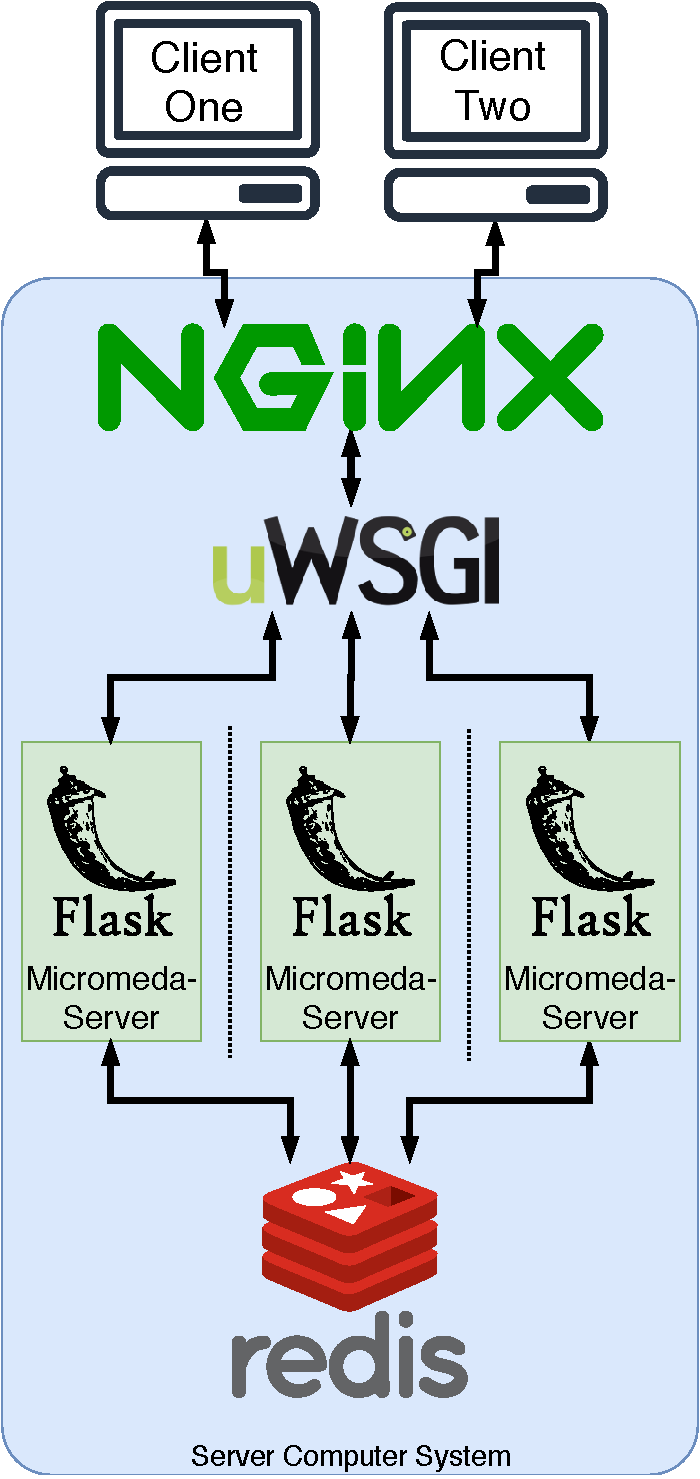
\includegraphics[width=0.40\textwidth]{media/micromeda-medium-deployment.pdf}
	 \caption{When deployed to the handle traffic of multiple users, Micromed-Server's Python code is placed behind a HTTP server and WSGI middleware server. Multiple copies of the Python code can then run simultaneously. Redis is used to provide shared data between these processes. Note the genomeProperties.txt files and default Micromeda files have been omitted for simplicity.}
	 \label{fig:micromeda-medium-deploy}
\end{figure}

\subsection{Multiple Server Deployment}

For a large number of simultaneous users, Micromeda-Server may need to be scaled to multiple servers. This is done placing a load balancer out front of multiple copies of the above deployment running on separate server computer systems. Redis can also be placed on its own server computer system or its on computer cluster. This deployment can be easily scaled horizontally by adding new server computer systems.

\begin{figure}[!ht]
  \centering
	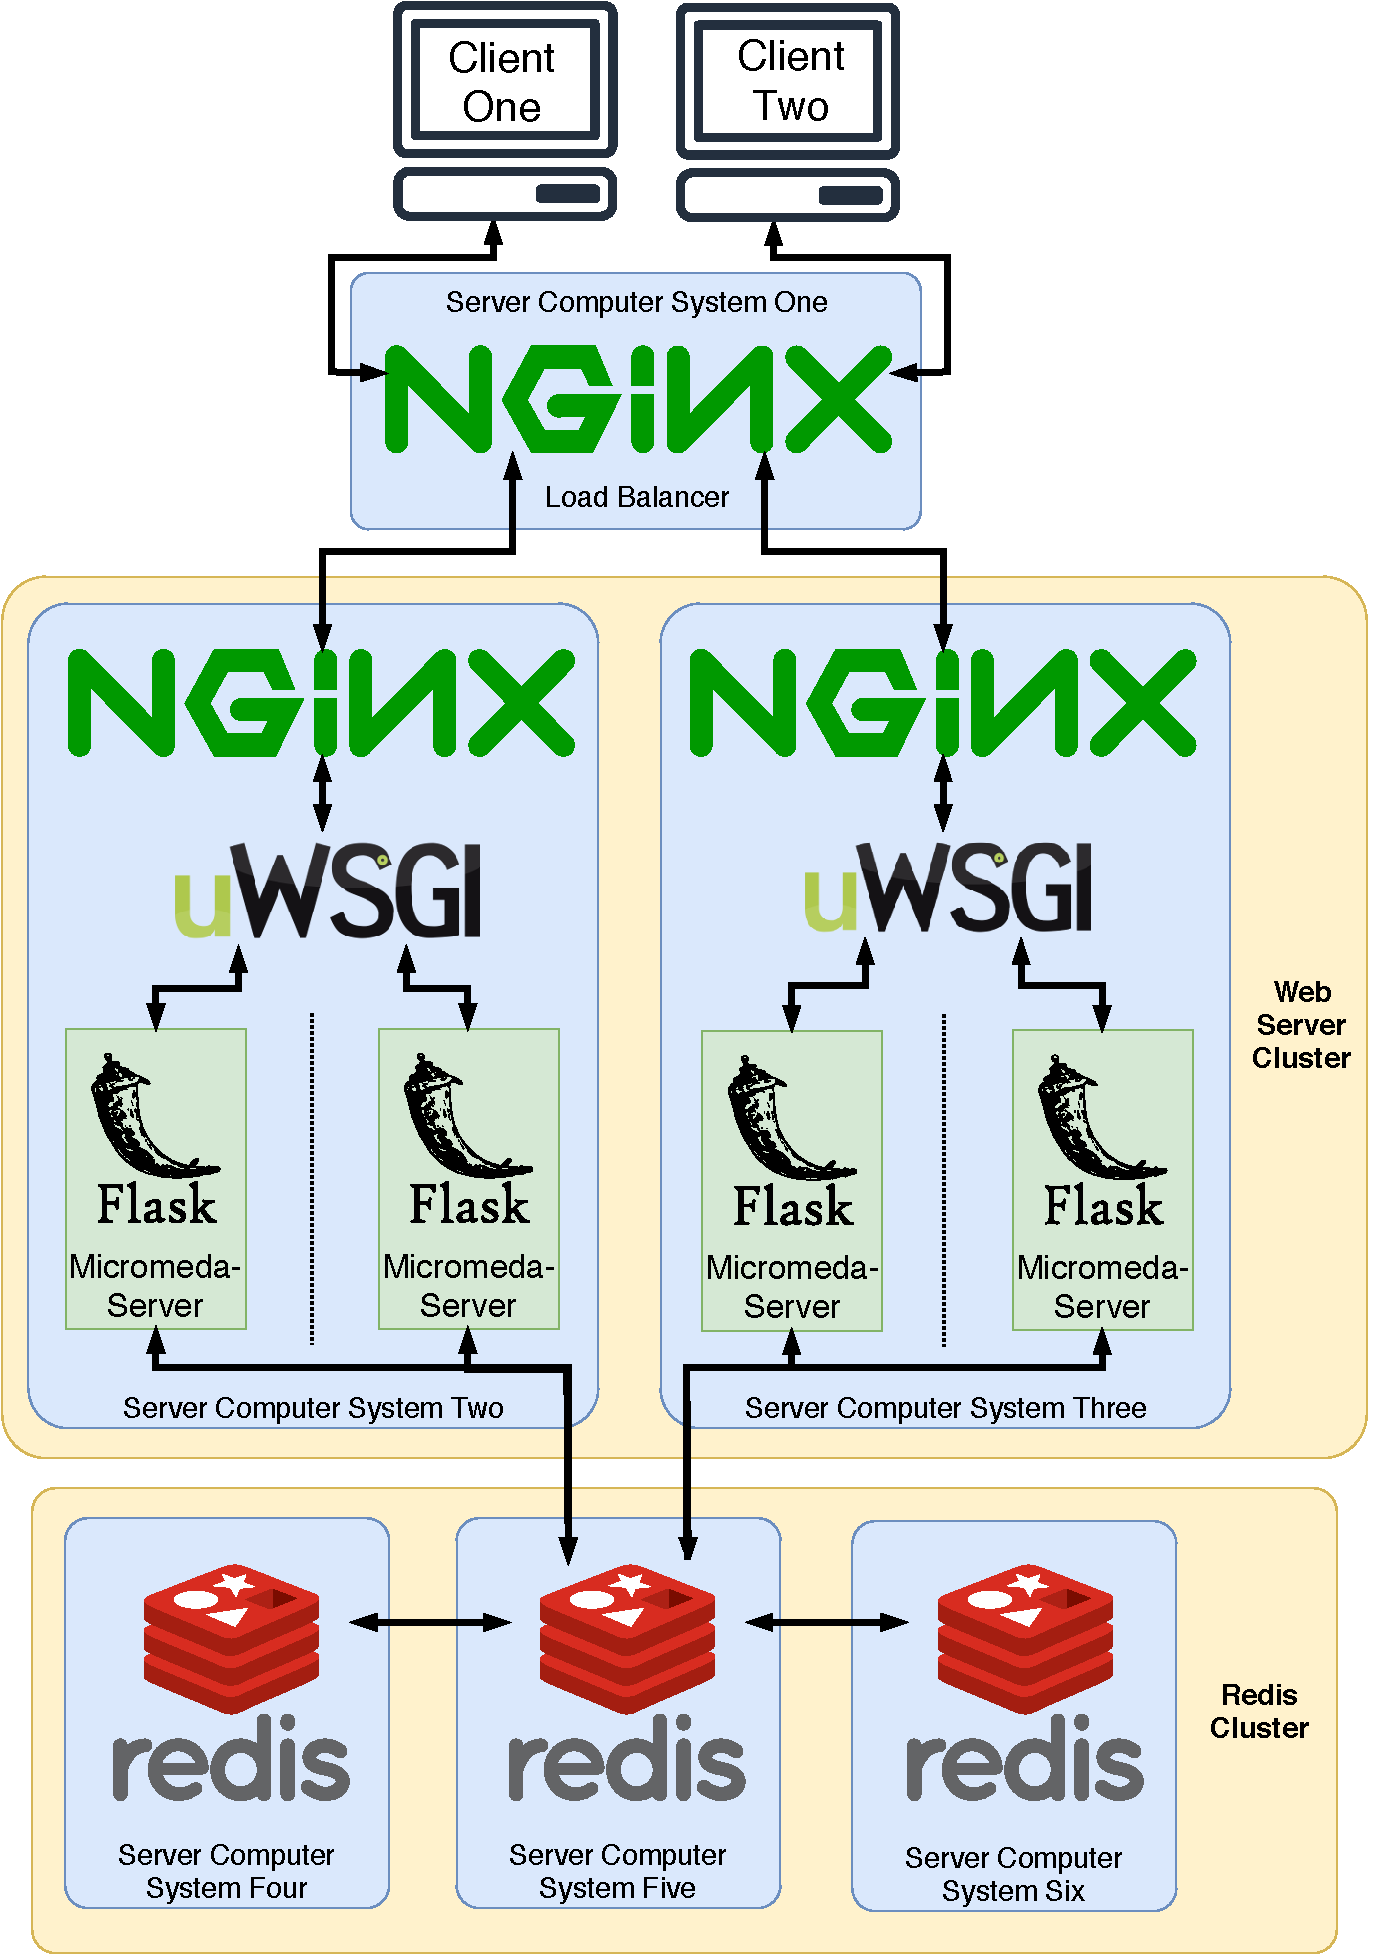
\includegraphics[width=0.50\textwidth]{media/micromeda-heavy-deployment.pdf}
	 \caption{When Micromeda is required to scale to handle hundreds or thousands of simultaneous users, its workload must be spread out across multiple web and caching server computer systems. The performance of such deployments can be increased by adding hardware to either the caching or web server clusters. Note that a copy of the genomeProperties.txt file and default Micromeda file would be stored on each computer in the web server cluster and have been omitted for simplicity.}
	 \label{fig:micromeda-large-deploy}
\end{figure}

\subsection{Cloud Platform As A Service (PaaS) Deployment}

Various cloud computing corporations have developed Platform as a Service (PaaS) \cite{lawton2008developing} products (see \href{en.wikipedia.org/wiki/Platform\_as\_a\_service}{en.wikipedia.org/wiki/Platform\_as\_a\_service}) that help users scale Python web applications without having to spend the time setting up a complex multiple server deployment. These PaaS, for example Google App Engine (\href{cloud.google.com/appengine}{cloud.google.com/appengine}) or Heroku (\href{heroku.com}{heroku.com}), provide the simplicity of a single user deployment with the scalability of a multiple server deployment. They do this by only requiring the developers to upload their Flask Python code and automate the rest of the deployment process. For example, the creation of load balancers and multiple copies of request handling processes. They perform these tasks in the background and invisibly to developer who uploaded their code. Such platforms can also be set up to pull new versions of Micromeda-Server directly from its Github repository upon their release, allowing for the continually update of the deployment's Python code to latest version. PaaS systems also allow for the deployment of Redis clusters, for example Google's Cloud Memorystore (see \href{cloud.google.com/memorystore/}{google.com/memorystore}).

\section{Future Improvements} \label{micromeda-server-improvements}

Micromeda-Server currently provides endpoints for all the necessary types of information needed by Micromeda's web-based visualization client. However, in addition to the existing endpoints, new endpoints could be made that would provide new data for future versions of this client, allowing it to have expanded functionality. Performance optimizations for the existing endpoints could also be made which could reduce latency in client's user interface by reducing the time it needs to wait for responses from Micromeda-Server. Improvements to Micromed-Server's existing endpoints and a potential new endpoint are discussed below.

\subsection{Improving Performance of the Upload Endpoint}

The \textbf{upload} endpoint takes a Micromeda file and saves its contents to a Redis cache. This endpoint was shown to have poor performance (see Section \ref{micromeda-server-performance}) and should be optimized to make the endpoint respond faster. Most of the performance problems with this endpoint can be attributed to the performance of parsing Micromeda files into GenomePropertiesResultsWithMatches objects using the \textbf{load\_assignment\_caches\_from\_database \\ \_with\_matches} function of Pygenprop's results module. The performance of this function was also found to be poor (see Section \ref{micromeda-file-performance}). Performance improvements to this function are discussed in detail in Section\ref{micromeda-file-improvements}. The performance optimisations recommended in Section \ref{micromeda-file-improvements} should be adopted and should drastically improve the performance of the endpoint. 

In addition to improvements to Pygenprop, some performance gains could be made by having the endpoint code skip writing newly uploaded Micromeda files to disk before parsing. Instead, the uploaded file could be parsed as it its streamed into main memory. This would remove the latency of writing the file to disk and then reading it back again. Temporarily writing and then deleting every uploaded file to disk could also put much wear and tear on the hard disks of the server computer system on which Micromeda-Server is running on. Using MessagePack instead of SQLite3 for the Micromeda file format, as discussed in Section \ref{micromeda-file-performance}), would make implementing such stream processing easier. In general, SQLite3 files can only be opened from a file on disk, not in-memory streams, unlike MessagePack. If MessagePack is not chosen as an alternate format, an altertnive would be to write the uploaded SQLIite3 Micromeda file to a Random-Access Memory Disk (see \href{en.wikipedia.org/wiki/RAM\_drive}{en.wikipedia.org/wiki/RAM\_drive}) before parsing.

\subsection{Improving Performance of the Get_Tree Endpoint}

As mentioned in Subsubsection \ref{pygenprop-json-serialization}, Pygenprop's serialization of GenomePropertiesResults objects to JSON, via GenomePropertiesResultsWithMatches object's to_json method, is quite slow. This JSON serialization method is used by Micromeda-Server's \textbf{get_tree} endpoint (see Subsection \ref{get-tree}) and may be the source of the endpoints poor performance as discussed in Section \ref{micromeda-server-performance}. The optimizations suggested in Subsubsection \ref{pygenprop-json-serialization} should greatly improve this endpoints performance. The performance of \textbf{get_tree} endpoint could also be improved by caching the JSON generated by the endpoint to Redis. On subsequent API calls the cached tree could be recalled from Redis instead and returned to the client instead of being regenerated with every call. On having to generate the tree once would drastically improve the endpoint performance.

\subsection{Creation of an Endpoints for Returning Property and Step Assignments}

One of the suggestions in Subsubsection \ref{Subsubsection \ref{pygenprop-json-serialization}}, which could improve JSON serialization performance of GenomePropertiesResultsWithMatches, objects was to reconfiguring the structure of its \textbf{to\_json}'s method's output. Specifically, to move per-organism assignments from each node on the JSON tree to a secondary hash table placed alongside it in the same JSON document. The author notes that such a hash table of organism property assignments could be returned in by its own endpoint rather than being part of the tree JSON returned by Micromeda-Server's \textbf{get_tree} endpoint. An endpoint could also be made for returning step assignment results. Having three endpoints to access data from a stored Micromeda file would follow a policy of Separation of Concerns (SoC) (see \href{en.wikipedia.org/wiki/Separation\_of\_concerns}{en.wikipedia.org/wiki/Separation\_of\_concerns}) and would allow client applications which only need the property tree, but not property assignments, to get their genome property tree more rapidly. It would be prudent to refactor (\href{en.wikipedia.org/wiki/Code\_refactoring}{en.wikipedia.org/wiki/Code\_refactoring}) Pygenprop's GenomePropertiesResultsWithMatches and GenomePropertiesResults objects to add methods which could be used to generate JSON documents containing only property or step assignments. Such methods could be used by these endpoints returning step and property assignments. Such refactorings could use pandas DataFrame's \textbf{to_json} method for rapidly convert these object's \textbf{property_result} and \textbf{step_result} DataFrames to JSON.

\subsection{Creation of an Endpoint for Returning Domain Annotation Supporting Property Steps}

Micromeda files not only contain property and step assignments for a set of organisms, but also contains supporting information such as domain annotations and proteins sequences which support the existence of property steps. Micromeda-Server currently provides an endpoint for accessing protein sequences which support steps (see Subsection \ref{get-fasta-endpoint}). However, there are no endpoint for accessing the stored InterProScan annotations of these proteins. Specifically, these annotations contain E-value scores representing how closely the domain in the protein matches a model of a representative domain in a protein database. These E-value scores may be useful for client web application visualization compare not only the presence and absence of proteins which support property steps but also compare how close these matches are to existing domain models. Thus, it may useful to create a new endpoint which returns these domain annotation E-value scores. This endpoint could generated its data from the \textbf{step_matches} DataFrame of reconstituted GenomePropertiesResultsWithMatches objects. 

\section{Summary}

The creation of web server API's for accessing information about biochemical pathways, and even the pre-calculated presence and absence of these pathways across organisms, is quite common. Indeed, such web APIs have been developed by the both the creators of KEGG and Metacyc, not only for their own web applications but also for public use. A web API was also generated for EBI's Genome Properties database website. However, its API is not publicly available and is only designed to support the website. 